% !TeX spellcheck = it_IT
%Carattere dimensione 12
\documentclass[12pt]{report}

%Margini e interlinea
\usepackage[top=1in, bottom=1in, left=1.2in, right=1in]{geometry}
\pagestyle{plain}
\linespread{1.5}

%Librerie utili
\usepackage[italian]{babel} % conversione in italiano
\usepackage[utf8]{inputenc}
\usepackage{libertine}
\usepackage{graphicx}
\usepackage{floatflt}
\usepackage{blindtext}
\usepackage{enumitem}
\usepackage{amsthm}
\usepackage{subfig}
\usepackage{listings}
\usepackage{listingsutf8}
\usepackage{amsmath}
\usepackage{framed}
\usepackage{minibox}
\usepackage{float}
\usepackage{wrapfig}
\usepackage{longtable}
\usepackage[strict]{changepage}
\usepackage{pgfplots}
\usepackage[utf8]{inputenc}


\pgfplotsset{width=11cm,compat=1.9}
\usepgfplotslibrary{external}

% \tikzexternalize
% \usetikzlibrary{positioning}

\usepackage{standalone}
\usetikzlibrary{positioning}

\begin{document}

\begin{titlepage}
  \begin{figure}[t]
    %\centering
\includegraphics[width=0.9\textwidth]{marchio-unipi.eps}
    \centering
\includegraphics[width=0.9\textwidth]{./img/logo.eps}
    \vspace{1cm}
    
    \centering
\includegraphics[width=0.4\textwidth]{./img/cherubino.eps}
  \end{figure}

  \begin{center}
    \textbf{ Dipartimento di Informatica\\ Corso di Laurea Triennale in Informatica\\}
    \vspace{15mm}
    {\LARGE{\bf Localizzazione Indoor Basata su Beacon Bluetooth a Bassa Potenza
    Attraverso Tecniche di Deep Learning}}\\
    % \vspace{3mm}
    % {\LARGE{\bf Attraverso Tecniche di Deep Learning}}\\
    {{\bf un progetto realizzato per Consorzio Metis e ASL Toscana}} \\
  \end{center}

  \vspace{20mm}

  \begin{minipage}[t]{0.47\textwidth}
    {\large{\bf Relatori:\\ Prof. Gianluigi Ferrari 
    % \\ Prof. Alessio Micheli
    }}
  \end{minipage}\hfill\begin{minipage}[t]{0.47\textwidth}\raggedleft
    {\large{\bf Presentata da: \\ Marco Pampaloni \\ }}
  \end{minipage}

  \vspace{18mm}

  \centering{\large{\bf Sessione Estiva \\ Anno Accademico 2019/2020 }}

\end{titlepage}

\tableofcontents

\begin{abstract}
  \begin{figure}
    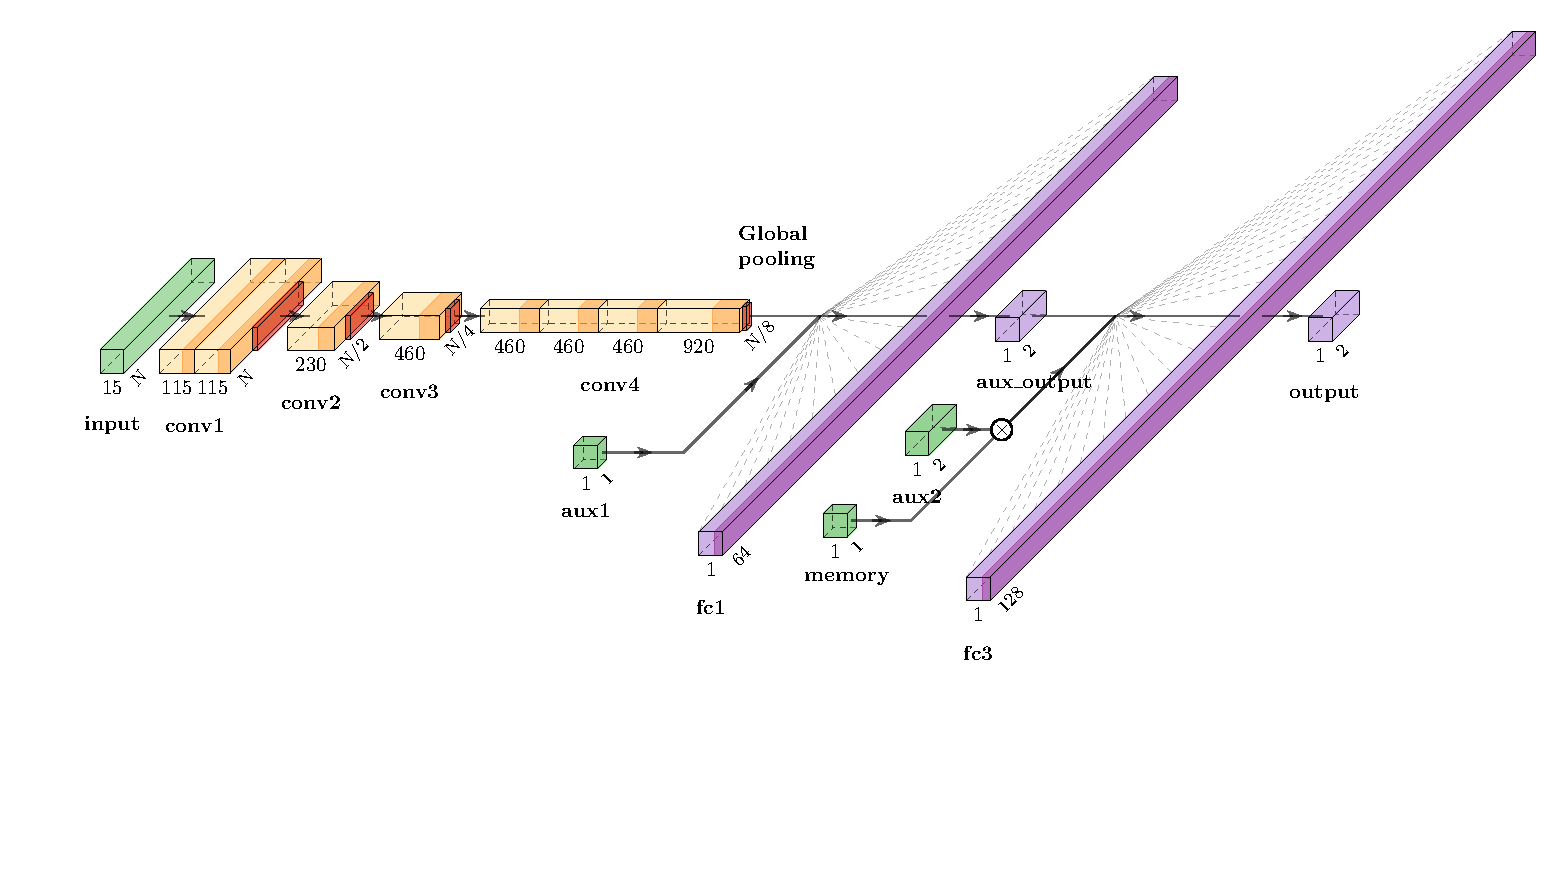
\includegraphics[width=\textwidth]{./img/architettura.pdf}
    \caption{Architettura Neurale}
  \end{figure}
  \documentclass{standalone} 
\begin{document}
% \section{Background}
Il problema della Localizzazione Indoor si è rivelato di particolare interesse
pratico negli ultimi anni. Questa tesi mostra come moderne tecniche di Deep
Learning possano risultare determinanti nella corretta risoluzione di tale
problema.
\\
% \section{Methods}
L'approccio analizzato sfrutta una rete neurale convoluzionale (CNN) profonda:
l'input del modello è caratterizzato da una serie temporale di segnali
broadcast \emph{Bluetooth Low Energy} (BLE) emessi da un insieme di Beacon
disposti all'interno dell'edificio adibito alla Localizzazione Indoor, mentre
l'output è una coppia di coordinate relative alla posizione all'interno
dell'edificio stesso. Sono state inoltre utilizzate varie tecniche di
\emph{data augmentation} per produrre un dataset di grandi dimensioni sulla
base dei campionamenti dei segnali effettuati in loco.
\\
% \section{Results}
A seguito dell'addestramento, il modello utilizzato ha mostrato un errore medio
assoluto (MAE) sul dataset di test pari a \emph{30cm}, esibendo una discreta
affidabilità anche rispetto a variazioni significative dei segnali dovute al
rumore ambientale. Un ensemble di modelli, ognuno addestrato con diversi
iperparametri, ha permesso di ridurre l'errore medio fino a circa \emph{26cm}.
\\
Il modello prodotto risulta eseguibile in tempo reale su dispositivi
mobile con ridotte capacità computazionali, rendendolo particolarmente adatto
alla 
% \section{Conclusion}
così detta navigazione \emph{``blue-dot``} all'interno di contesti Indoor.
Tuttavia si evidenzia come la variazione dell'output del modello possa
risultare in una navigazione poco fluida. Per arginare questo problema viene
applicato un filtro di Kalman al modello e viene sfruttato il sensore inerziale
dello smartphone per produrre un'euristica utile a individuare i movimenti
dell'utente.  
\end{document}

\end{abstract}

\chapter{Introduzione}

\chapter{Localizzazione Indoor}
\section{Introduzione al problema}
\section{Possibili soluzioni}
\section{Beacon BLE}
\section{RSSI e propagazione del segnale}
\section{Variabilità e rumore di fondo: requisiti di usabilità}
\section{Installazione dei Beacon e Acquisizione dei Dati}

\chapter{Deep Learning}
\section{Neurone Artificiale: Perceptron}
\section{Multi Layer Perceptron}
\section{Attivazione: ReLU e Funzioni Sigmoidee}
\section{Apprendimento: Metodo del Gradiente e BackPropagation}
\section{Reti Neurali Convoluzionali}
\section{Regolarizzazione}
\subsection{Overfitting e Underfitting}
\subsection{Regolarizzazione L2}
\subsection{Dropout}
\section{Dataset Augmentation e Preprocessing}
\subsection{Jittering}
\subsection{Ridimensionamento (Scaling)}
\subsection{Magnitude Warping}
\subsection{Permutazione di Sottoinsiemi (Subset Shuffling)}
\subsection{Deattivazione Selettiva}


\chapter{Architettura Software}
\section{TensorFlow}
\section{Keras}
\section{Google Colab}
\section{Weights \& Biases}
\section{Modello di Apprendimento}
\subsection{Input del Modello}
\subsection{Blocco Convoluzionale}
\subsection{Uso della Bussola e Output Ausiliario}
\subsection{Coefficiente di Memoria Residua e Input Ausiliario}
\subsection{Output del Modello}
\section{Addestramento del Modello}
\section{Ensembling}
\section{Compilazione e Deploy del Modello}

\chapter{Applicazione Mobile}
\section{Flutter}
\section{Planimetrie e Poligoni}
\section{Backend TensorFlow}
\subsection{TensorFlow Lite}
\subsection{Implementazione del Bridge di Comunicazione}
\section{Stabilizzazione del Modello}
\subsection{Utilizzo di Sensori Inerziali}
\subsection{Filtro di Kalman}

\chapter{Conclusioni}
\section{Risultati Sperimentali}
\subsection{Metriche di Errore: MSE, MAE, MaxAE}

\section{Lavori futuri}
\subsection{Input a Lunghezza Variabile}
\subsection{Reti Neurali Residuali}
\subsection{Variational Autoencoder: Generazione di nuovi dati}
\subsection{Transfer Learning}
\subsection{Input Masking e Ricostruzione dei Segnali}
\subsection{Transformers per Problemi di Regressione}
\subsection{Simulatore BLE}
\subsection{Posizionamento Magnetico}

\appendix

\bibliography{references}
\bibliographystyle{plain}

\end{document}
